\documentclass{article}

\usepackage{fancyhdr}
\usepackage{wrapfig}
\usepackage{extramarks}
\usepackage{multicol}
\usepackage{amsmath}
\usepackage{amsthm}
\usepackage{amsfonts}
\usepackage{tikz}
\usepackage{forest,adjustbox}
\usepackage[plain]{algorithm}
\usepackage{algpseudocode}
\usepackage{enumerate}
\usepackage[shortlabels]{enumitem}                     
          \setlist[enumerate, 1]{1\textsuperscript{o}}



\usepackage{listings}
\usepackage{xcolor}
%\lstset { %
%  language=C++,
%  backgroundcolor=\color{black!5}, % set backgroundcolor
%  basicstyle=\footnotesize,% basic font setting
%}

%\usetikzlibrary{automata,positioning}
\usetikzlibrary{positioning,shapes,shadows,arrows,automata} %
% Basic Document Settings
%

\topmargin=-0.45in
\evensidemargin=0in
\oddsidemargin=0in
\textwidth=6.5in
\textheight=9.0in
\headsep=0.25in

\linespread{1.1}

\pagestyle{fancy}
\lhead{\hmwkClass}
\chead{ (\hmwkClassInstructor\ \hmwkClassTime) }
\rhead{\shortName \hspace{0.4cm} \hmwkTitle}
\lfoot{\lastxmark}
\cfoot{\thepage}

\renewcommand\headrulewidth{0.4pt}
\renewcommand\footrulewidth{0.4pt}

\newcommand\curl[1]{\{#1\}}

\setlength\parindent{0pt}

%
% Create Problem Sections
%

\newcommand{\enterProblemHeader}[1]{
  \nobreak\extramarks{}{Problem \arabic{#1} continued on next page\ldots}\nobreak{}
  \nobreak\extramarks{Problem \arabic{#1} (continued)}{Problem \arabic{#1} continued on next page\ldots}\nobreak{}
}

\newcommand{\exitProblemHeader}[1]{
  \nobreak\extramarks{Problem \arabic{#1} (continued)}{Problem \arabic{#1} continued on next page\ldots}\nobreak{}
  \stepcounter{#1}
  \nobreak\extramarks{Problem \arabic{#1}}{}\nobreak{}
}

\setcounter{secnumdepth}{0}
\newcounter{partCounter}
\newcounter{homeworkProblemCounter}
\setcounter{homeworkProblemCounter}{1}
\nobreak\extramarks{Problem \arabic{homeworkProblemCounter}}{}\nobreak{}

%
% Homework Problem Environment
%
% This environment takes an optional argument. When given, it will adjust the
% problem counter. This is useful for when the problems given for your
% assignment aren't sequential. See the last 3 problems of this template for an
% example.
%
\newenvironment{homeworkProblem}[1][-1]{
  \ifnum#1>0
    \setcounter{homeworkProblemCounter}{#1}
  \fi
  \section{Problem \arabic{homeworkProblemCounter}}
  \setcounter{partCounter}{1}
  \enterProblemHeader{homeworkProblemCounter}
}{
  \exitProblemHeader{homeworkProblemCounter}
}

%
% Homework Details
%  - Title
%  - Due date
%  - Class
%  - Section/Time
%  - Instructor
%  - Author
%

\newcommand{\hmwkTitle}{Homework\ \#3}
\newcommand{\hmwkDueDate}{February 10 2016}
\newcommand{\hmwkClass}{CS581 Theory of Computation}
\newcommand{\hmwkClassTime}{Winter 2016}
\newcommand{\hmwkClassInstructor}{Harry H. Porter}
\newcommand{\hmwkAuthorName}{Konstantin Macarenco}
\newcommand{\shortName}{Konstantin M.}

%
% Title Page
%

\title{
  \vspace{2in}
  \textmd{\textbf{\hmwkClass:\ \hmwkTitle}}\\
  \normalsize\vspace{0.1in}\small{Due\ on\ \hmwkDueDate\ at 2:00pm}\\
  \vspace{0.1in}\large{\textit{\hmwkClassInstructor\ \hmwkClassTime}}
  \vspace{3in}
}

\author{\textbf{\hmwkAuthorName}}
\date{}

\renewcommand{\part}[1]{\textbf{\large Part \Alph{partCounter}}\stepcounter{partCounter}\\}
\newcommand{\answ}[1]{\hspace{1cm}\textbf{Answ:} #1}
\newcommand{\problem}[1]{\large{\textbf{Problem #1}}\\}

%
% Various Helper Commands
%

% Useful for algorithms
\newcommand{\alg}[1]{\textsc{\bfseries \footnotesize #1}}

% For derivatives
\newcommand{\deriv}[1]{\frac{\mathrm{d}}{\mathrm{d}x} (#1)}

% For partial derivatives
\newcommand{\pderiv}[2]{\frac{\partial}{\partial #1} (#2)}

% Integral dx
\newcommand{\dx}{\mathrm{d}x}

% Alias for the Solution section header
\newcommand{\solution}{\textbf{\large Solution}}

% Probability commands: Expectation, Variance, Covariance, Bias
\newcommand{\E}{\mathrm{E}}
\newcommand{\Var}{\mathrm{Var}}
\newcommand{\Cov}{\mathrm{Cov}}
\newcommand{\Bias}{\mathrm{Bias}}

\newcommand\Vtextvisiblespace[1][.3em]{%
  \mbox{\kern.06em\vrule height.3ex}%
  \vbox{\hrule width#1}%
  \hbox{\vrule height.3ex}}

\begin{document}

\maketitle

\pagebreak

\begin{homeworkProblem}
Provide a  formal description of Turing Machines. \\

A Turing machine is a 7-tuple, $(Q,\Sigma,\Gamma,\delta,q_0,q_{accept}, q_{reject})$, where $Q,\Sigma, \Gamma$ are all finite setns and.
\begin{enumerate}[1., leftmargin = 0.8cm]
\itemsep0em
\item $Q$ is the set of states,
\item $\Sigma$ is the input alphabet not containing the \textbf{blank symbol} $\Vtextvisiblespace[0.2cm]$
\item $\Gamma$ is the tape alphabet, where $\Vtextvisiblespace[0.2cm] \in \Gamma$ and $\Sigma \subseteq \Gamma$,
\item $\delta: Q\times \Gamma \rightarrow Q \times \Gamma \times \curl{L,R}$ is t he transition function,
\item $q_0 \in Q$ is the start state,
\item $q_{accept} \in Q$ is the accept state, and
\item $q_{reject} \in Q$ is the reject state, where $q_{reject} \neq q_{accept}$.
\end{enumerate}

\end{homeworkProblem}

\begin{homeworkProblem}
Describe  informally (no more  than  half  a  page)  the operation  of a  Turing Machine. \\

Turing machine consists of infinite tape (unlimited memory), and a tape head that can move
left and right and read and write symbols from/to the tape.
\end{homeworkProblem}

\begin{homeworkProblem}
Design a  Turning Machine that  takes  3  numbers in unary  representation and adds  
them  together,  leaving the result on the tape.  (Unary representation:$5$ in unary  is 
$“11111”$).  Assume the three  numbers are separated  by the $“\#”$ symbol. For example,  
the problem $3+4+2$  would  be represented on the tape  as: $111\#1111\#11$ the 
machine should accept with  the following  string on the tape: $111111111$. Give  your  
machine in graph  notation,  in the style  of Figure $3.8$. \\

Machine M that recognizes this language is simple, since we now upfront that 3 numbers 
are added separated by two $\#$. Machine $M$ works as follows:\\

``On input $w$:
\begin{enumerate}[1., leftmargin = 1.5cm]
\itemsep0em
\item read until the end of the input, replacing 1s and $\#$ with 1s, if see any other symbol fail.
\item erase last two 1s with blanks by moving right, and accept.
\end{enumerate}

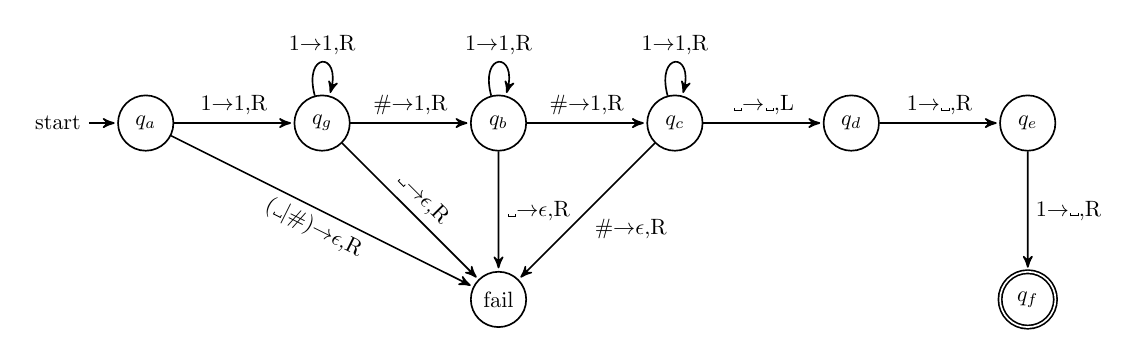
\begin{tikzpicture}[->,>=stealth',shorten >=1pt,auto,node distance=2.8cm,
                    semithick, transform shape, scale = 0.8]
  \tikzstyle{every state}=[fill=none,draw=black,text=black]

  \node[initial,state]     (A)                    {$q_a$};
  \node[state]             (G) [right of=A]       {$q_g$};
  \node[state]             (B) [right of=G]       {$q_b$};
  \node[state]             (C) [right of=B]       {$q_c$};
  \node[state]             (D) [right of=C]       {$q_d$};
  \node[state]             (E) [right of=D]       {$q_e$};
  \node[state,accepting]   (F) [below of=E]       {$q_f$};
  \node[state]             (Z) [below of=B]       {fail};

  \path (A) edge              node [align=center]{1$\rightarrow$1,R} (G)
            edge [sloped,below] node [align=center] {($\textvisiblespace|\#$)$\rightarrow$$\epsilon$,R} (Z)
        (G) edge [loop above] node [align=center] {1$\rightarrow$1,R} (G)
            edge [sloped] node [align=center] {$\textvisiblespace$$\rightarrow$$\epsilon$,R} (Z)
            edge              node [align=center] {$\#$$\rightarrow$$1$,R} (B)
        (B) edge [loop above] node [align=center] {1$\rightarrow$1,R} (B)
            edge              node [align=center] {$\textvisiblespace$$\rightarrow$$\epsilon$,R} (Z)
            edge              node [align=center] {$\#$$\rightarrow$$1$,R} (C)
        (C) edge [loop above] node [align=center] {1$\rightarrow$1,R} (C)
            edge              node [align=center] {$\textvisiblespace$$\rightarrow$$\textvisiblespace$,L} (D)
            edge              node [align=center] {$\#$$\rightarrow$$\epsilon$,R} (Z)
        (D) edge              node [align=center] {1$\rightarrow$\textvisiblespace,R} (E)
        (E) edge              node [align=center] {1$\rightarrow$\textvisiblespace,R} (F);
\end{tikzpicture}

\end{homeworkProblem}

\begin{homeworkProblem}
What  is a  Decidable  Language? \\

A language $L$ is decidable (or Turing decidable) if there exists a Turing machine $M$ such that
on input $x$, $M$ accepts if $x \in L$, and $rejects$ otherwise.
\end{homeworkProblem}

\begin{homeworkProblem}
What  is a  Turing-Recognizable Language?\\

A language $L$ is recognizable (or Turing recognizable) if there exists a Turing machine $M$ such that
on input $x$, $M$ accepts if $x \in L$, but may either reject or loop forever otherwise.
\end{homeworkProblem}

\begin{homeworkProblem}
What  is a  Recursively Enumerable Language?\\

Same as Turing-recongnizable.
\end{homeworkProblem}

\begin{homeworkProblem}
State  the Church-Turing  Thesis. \\

Every effective calculation can be carried by a Turing Machine.\\
Effective calculation of a procedure M can be defined as:
\begin{enumerate}[1., leftmargin = 1.5cm]
\itemsep0em
\item M is set out in terms of a finite number of exact instructions (each instruction being expressed by means of a finite number of symbols);
\item M will, if carried out without error, produce the desired result in a finite number of steps;
\item M can (in practice or in principle) be carried out by a human being unaided by any machinery save paper and pencil;
\item M demands no insight or ingenuity on the part of the human being carrying it out.
\end{enumerate}

\end{homeworkProblem}

\problem{3.6}
In Theorem 3.21, we showed that a language is Turing-recognizable iff some enumerator
enumerates it. Why didn't we use the following simpler algorithm for the forward direction
of the proof? As before, $s_1,s_2,\cdots$ is a list of strings in $\Sigma^*$ \\

E = ``Ignore the input.
\begin{enumerate}[1., leftmargin = 1.5cm]
\itemsep0em
\item Repeat the following for $i = 1,2,3,\cdots$.
\item Run $M$ on $s_i$.
\item If it accepts, print ou t $s_i$''
\end{enumerate}

The problem with this definition is that if on step 2 M loops on some input 
$s_j$, then $E$ will fail to check any input after, in this case $E$ will
fail to enumerate the language.  \\
\problem{3.8}

Give implementation-level descriptions of Turing machines that decide the 
following languages over the alphabet $\curl{0,1}$

\problem{3.8   (b)}
$\curl{w | w \text{ contains twice as many 0s as 1s}}$ \\

\begin{enumerate}[1., leftmargin = 1.5cm]
\itemsep0em
\item Scan the tape for the first 0 that has not been marked, if 
none found, goto the last step, otherwise mark it.
\item Move to the next unmarked 0, if none reject, otherwise mark it and
move back to the start of the input.
\item Scan for the first unmarked 1, if none reject, otherwise mark it.
\item  Move the head to the beginning of the input, and goto step 1.
\item Move the head to the beginning of the input, and scan for unmarked
1s, if none accept, otherwise reject.
\end{enumerate}
\problem{3.9}
Let a k-$PDA$ be a pushdown automaton that has $k$ stacks. Thus a 0-$PDA$
is an NFA and a 1-$PDA$ is a conventional $PDA$. You already know that 1-$PDA$s
are more powerful (recognize a larger class of languages) htan 0-$PDA$s.
\begin{enumerate}[a., leftmargin = 1.5cm]
\itemsep0em
\item Show that 2-PDAs are more powerful than 1-PDAs.
\item Show that 3-PDAs are not more powerful than 2-PDAs.\\
    (Hint: Simulate a Turing machine tape with two stacks.)
\end{enumerate}

\begin{enumerate}[a., leftmargin = 1.5cm]
\itemsep0em
\item It is easy to show by example: 1-PDA is not powerful enough to recognize $L = \curl{a^n b^n c^n |
\text{ where } n \geq 0}$, but we can construct 2-PDA that will recognize $L$ as following:
\begin{enumerate}[1., leftmargin = 1.5cm]
\itemsep0em
\item Put all $a$ onto the first stack, and all $b$ onto the second stack.
\item When reading $c$ pop both stack simultaneously. Accept if input and both stack are empty, reject otherwise.
\item If encounter symbols out of order (b, c before a, or a between b and c) reject.
\end{enumerate}
\item To show that 3-PDAs are not more powerful than 2-PDAs, it is enough to show that
2-PDA can simulate a regular $TM$. \\
$TM$ can be simulated by a 2-PDA as follows:\\
First stack is responsible for handling everything on the left side of the TMs head, and right side
for handling everything on the right side of the TMs head. On every $M$ left transition $S$
$\delta(q_i,c_i) = (q_j,c_j,L)$ PDA pops $c_i$ off stack 2, pushes $c_j$ into stack 2, pops stack 1 and 
pushes the character into stack 2, and goes from state $q_i$ to $q_j$. Analogous for $\delta(q_i,c_i) = (q_j,c_j,R)$


\end{enumerate}
\problem{3.11}
A \textbf{Turing machine with doubly infinite tape} is similar to an ordinary
Turing machine, but its tape is infinite to the left as well as to the right. The tape
is initially filled with blanks except for the portion that contains the input. Computation is
defined as usual except that the head never encounters an end to the tape as it
moves leftward. Show that this type of Turing machine recognizes the class of Turing-recognizable 
languages. \\


\begin{enumerate}[1., leftmargin = 1.5cm]
\itemsep0em
\item It easy to show that \textbf{doubly infinite tape TM} can simulate regular $TM$ by not using the 
tape on the left side of the input.
\item \textbf{doubly infinite TM} can be easily simulated by \textbf{double tape TM}, by using second tape
as the left side of the \textbf{doubly infinite TM}, and since \textbf{ multi-tape TM} is equivalent to
regular $TM$ as it was proven in Sipser Theorem 3.13. \\
\end{enumerate}
\problem{3.15}
Show that the collection of decidable languages is closed under the operation of\\
\problem{3.15  (b)}
concatenation.\\

For any two decidable languages $L_1$ and $L_2$, let $M_1$ and $M_2$ be TMs that decide them.
Concatenation of two languages $L_1$ and $L_2$ is language $C = \curl{xy | \text{ where 
    } x \in L_1 \text{ and } y \in L_2}$.
We construct TM $M'$ that decides the concatenation of $L_1$ and $L_2$ that will non-deterministically 
split input $w$ into two $x$ and $y$, two check all possible combinations, i.e:\\

``On input $w$:
\begin{enumerate}[1., leftmargin = 1.5cm]
\itemsep0em
\item Non-deterministically split $w$ into $xy$.
\item Run $M_1$ on $x$, if $M_1$ rejects reject, otherwise goto next.
\item Run $M_2$ on $y$, if $M_2$ accepts accept, otherwise reject.
\end{enumerate}


\problem{3.15  (d)}
complementation.\\

For any decidable language $L$, let $M$ be TM that decides it.
We construct TM $M'$ that decides the complement  of $L$: \\

``On input $w$:
\begin{enumerate}[1., leftmargin = 1.5cm]
\itemsep0em
\item Run $M$ on $w$. If it rejects accept, otherwise reject. ''
\end{enumerate}

\end{document}
